\section{Tensors}
\subsection{Revision of IA}

In IA the concept of normal and shear stresses were covered. Normal stresses and shear stresses can be defined with the equations:
\begin{equation*}
\sigma = \frac{\mathbf{F}}{A} \hspace{5cm}  \tau = \frac{\mathbf{F}}{A}
\end{equation*}
where the forces and areas are defined by:
\begin{figure}[h!]
\centering
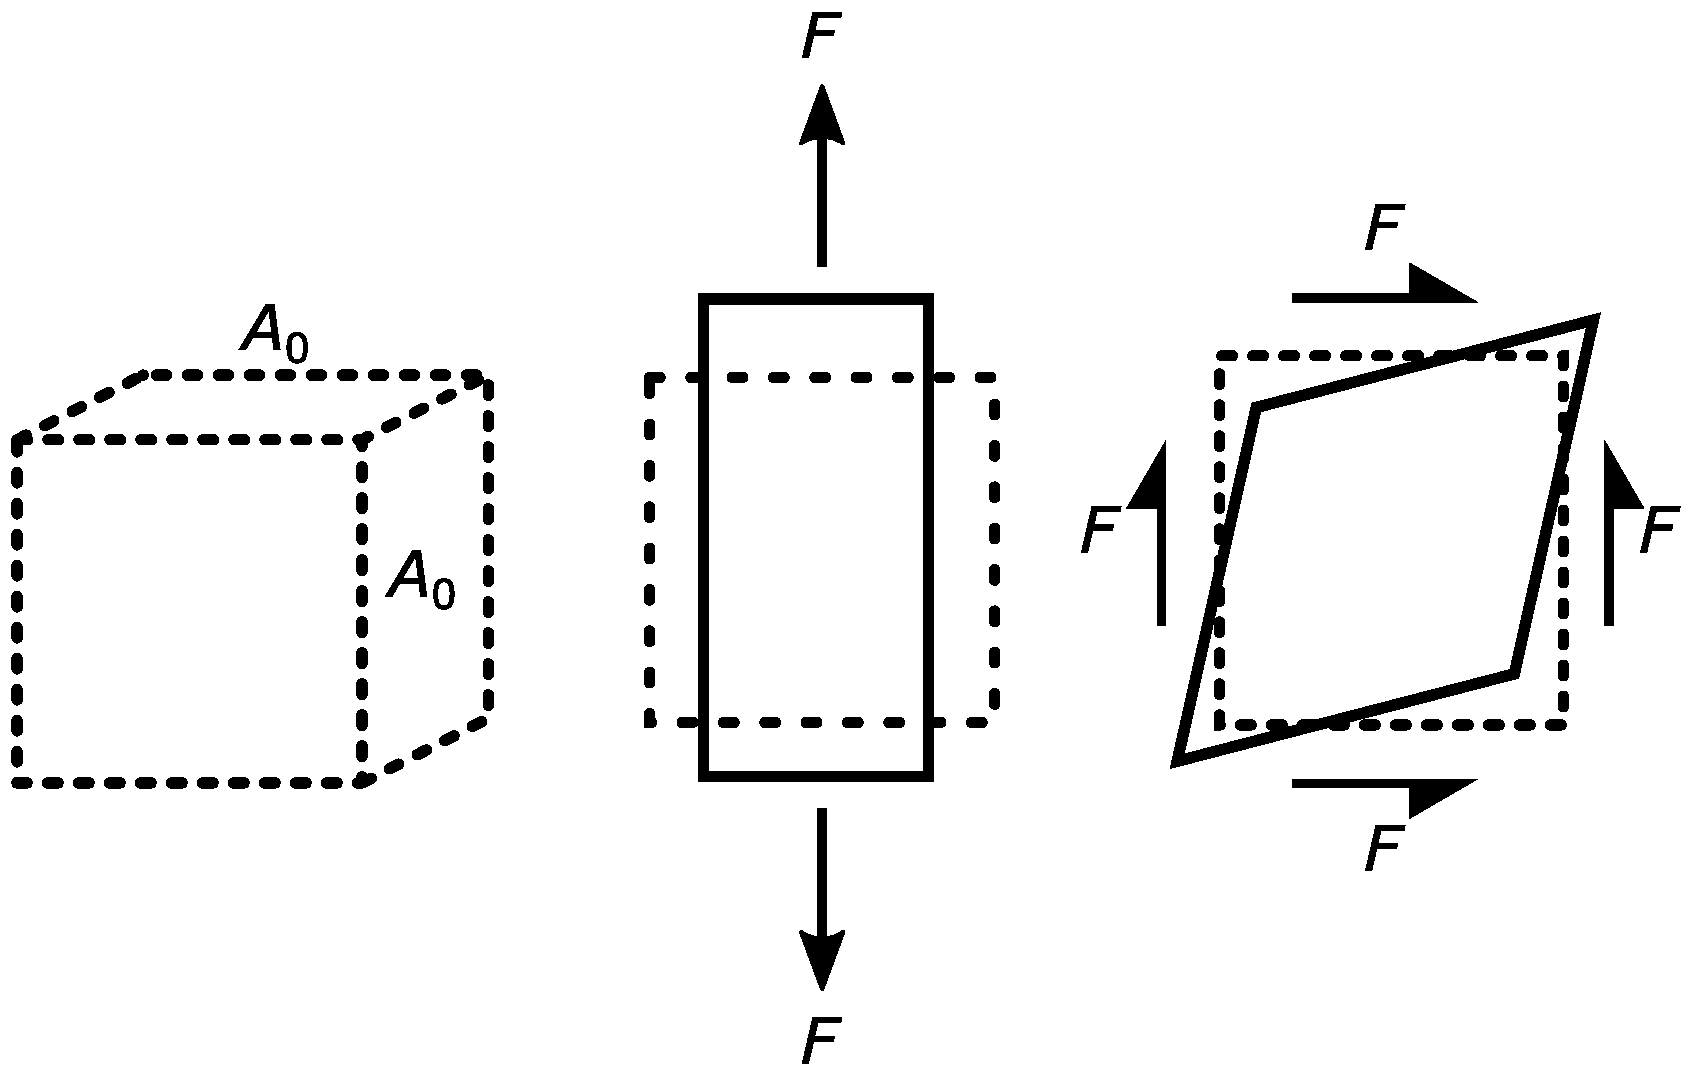
\includegraphics[width = 0.6\textwidth]{Stresses}
\end{figure}

The material will respond elastically as long as the stresses are below the failure stress, and we can define normal and shear strains:

\begin{equation*}
\varepsilon = \frac{\Delta x}{x_0} \hspace{5cm} \gamma = \frac{\Delta y}{x_0}
\end{equation*}
where the lengths are defined by:
\begin{figure}[h!]
\centering
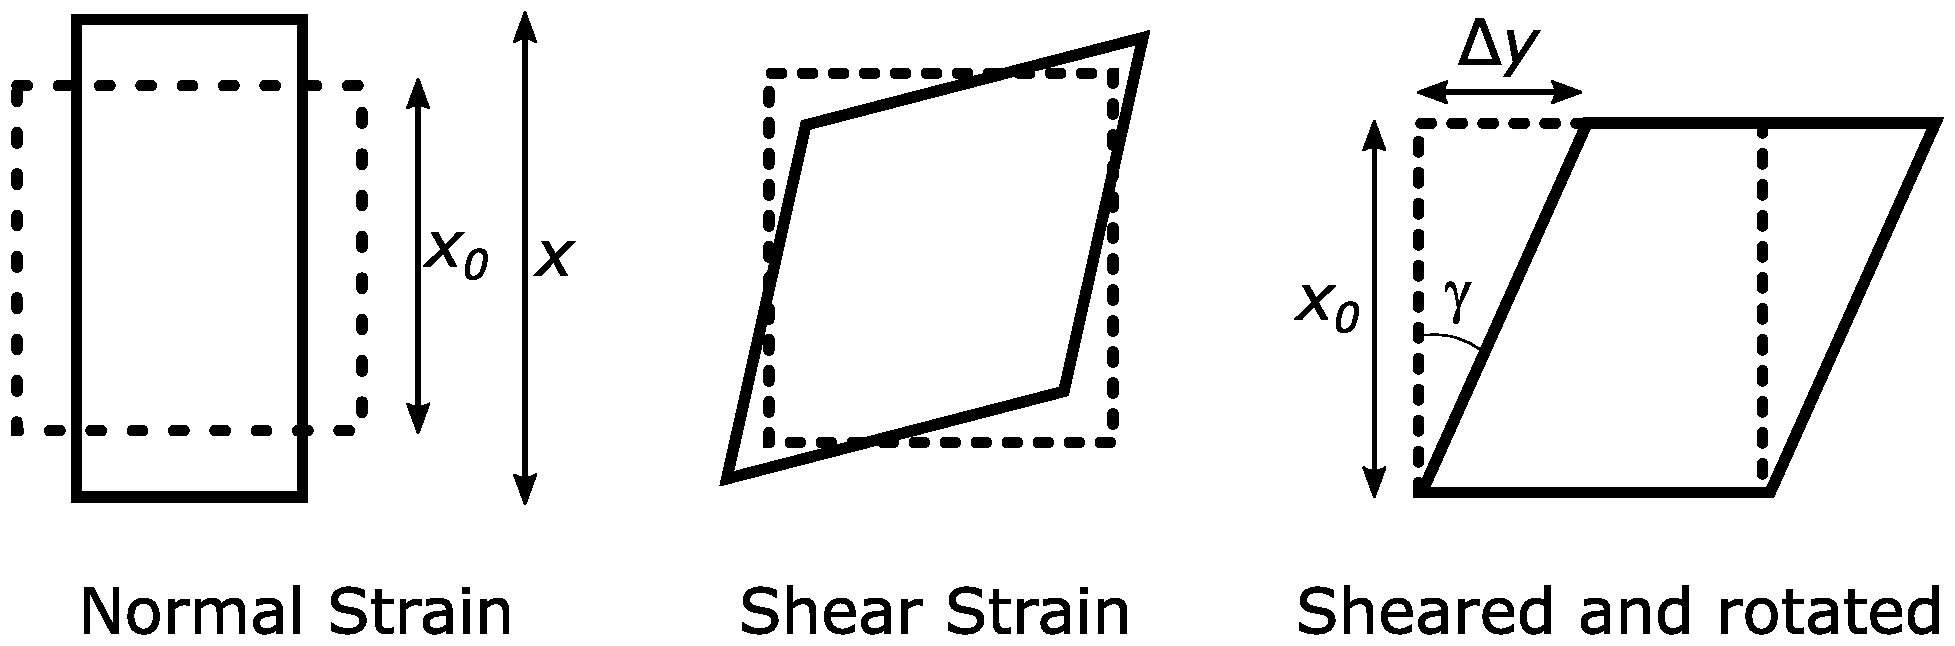
\includegraphics[width = 0.7\textwidth]{Strains}
\end{figure}

The quantities of stress and strain are linearly related for elastic behaviour and we can write:
\begin{align}
\sigma &= \varepsilon E \nonumber\\
\tau &= \gamma G \label{eqn:def_moduli}
\end{align}
where $E$ and $G$ are the Young's modulus and shear modulus respectively.

There are important points about this representation:
\begin{itemize}
\item For a general set of applied forces, both shear and normal stresses will develop, and furthermore the size of these components will vary as different sets of planes are considered, i.e.\ the frame of reference is important.
\item A stress or strain as defined above is implicitly defined by a magnitude and {\bf{two}} directions. For stress these are the direction that the force is acting in and the direction normal to the plane being considered. For strain these are the direction of displacement and the direction of the reference length.
\end{itemize}

Scalars and vectors are familiar concepts: scalars are defined by a magnitude, vectors are defined by magnitude and a single direction. Stress and strain cannot be completely described by scalars or vectors, and so cannot be resolved into components etc. Instead they can be described using tensors.


\subsection{Introduction to tensors}

A tensor is an $n$-dimensional array of values, where $n$ is the ``rank'' of the tensor. {\bf Scalars} and {\bf vectors} are \emph{zeroth} and \emph{first} rank tensors respectively. Properties that have no directionality and a single magnitude are scalars, and the concept of components does not apply.
\\
\\
\begin{annotation}
0\textsuperscript{th} rank tensors $\Longrightarrow$ Scalar quantities with no directionality.
\\
\\
Examples are temperature, density, energy, charge etc.
\end{annotation}
\\

A first rank tensor is a \emph{vector}. When represented as a tensor they have 3 values, or components, corresponding to the components in three mutually orthogonal directions. Each component can be thought of as having an index, usually written as a suffix. Several systems are used, such as \{$x,\,y,\,z$\} or \{$r,\,z,\,\theta$\}, here numerical suffices will be used: \{1,\,2,\,3\}. Vectors are then written
\begin{equation}
\mathbf{F} = F_i = [F_1,\, F_2,\, F_3]
\end{equation}
We will return to suffix notation, but the basic concept is as follows: wherever a suffix has a numerical value then the quantity refers to a specific component, e.g. $F_2$ is the magnitude of the component along the 2 axis, however where a suffix is a letter then this represents all the possible components, i.e. $F_i$ above is the  vector.
\\
\\
\begin{annotation}
1\textsuperscript{st} rank tensors $\Longrightarrow$ Vector quantities, a magnitude and direction and represented by a 1-D array with 3 components.
\\
\\
Examples are force, velocity, electric/magnetic field, polarisation, acceleration etc.
\end{annotation}

\subsubsection{Second rank tensors: Stress and Strain}

Stress and strain are examples of a second rank tensor, each component is defined in terms of two directions (e.g. the direction of the force and the normal of the plane upon which it acts defines a component of stress) and each component has two suffices, hence this is called a second rank tensor.
\\
\\
\begin{annotation}
2\textsuperscript{nd} rank tensors $\Longrightarrow$ tensors with a magnitude and two directions, represented by a 2-D array with 9 components. 
\\
\\
Examples are stress ($\sigma_{ij}$), strain ($\varepsilon_{ij}$), electrical resistivity ($\rho_{ij}$), thermal expansion coefficient ($\alpha_{ij}$) etc.
\end{annotation}

In each case the two suffices will have a physical interpretation. In the case of stress, the convention used here will be that the first suffix refers to the direction of the force being applied, and the second defines the normal of the plane upon which this force is acting (this convention can be reversed but as long as a single convention is used consistently then problems are unlikely). There are three directions in which a force or plane normal can lie, so there are nine combinations:

\begin{equation}
\sigma_{ij} = 
\begin{pmatrix}
\sigma_{11} & \sigma_{12} & \sigma_{13} \\
\sigma_{21} & \sigma_{22} & \sigma_{23} \\
\sigma_{31} & \sigma_{32} & \sigma_{33}
\end{pmatrix}\label{eqn:general_stress_tensor}
\end{equation}

For a component where $i$ and $j$ are equal, i.e. the main diagonal, the force acts perpendicular to the plane, and this component is a normal stress. Where $i$ and $j$ are not equal the force acts parallel to the plane and this component is a shear stress. For shear components the symbol $\tau_{ij}$ is sometimes used.
\\
\\


\begin{annotation}
$\sigma_{ii} \Longrightarrow $ Normal stress, force is parallel to plane normal

$\sigma_{ij} \Longrightarrow $ Shear stress, force is perpendicular to plane normal (sometimes written as $\tau_{ij}$)
\end{annotation}
\\
\\




\begin{figure}[bh!]
\centering
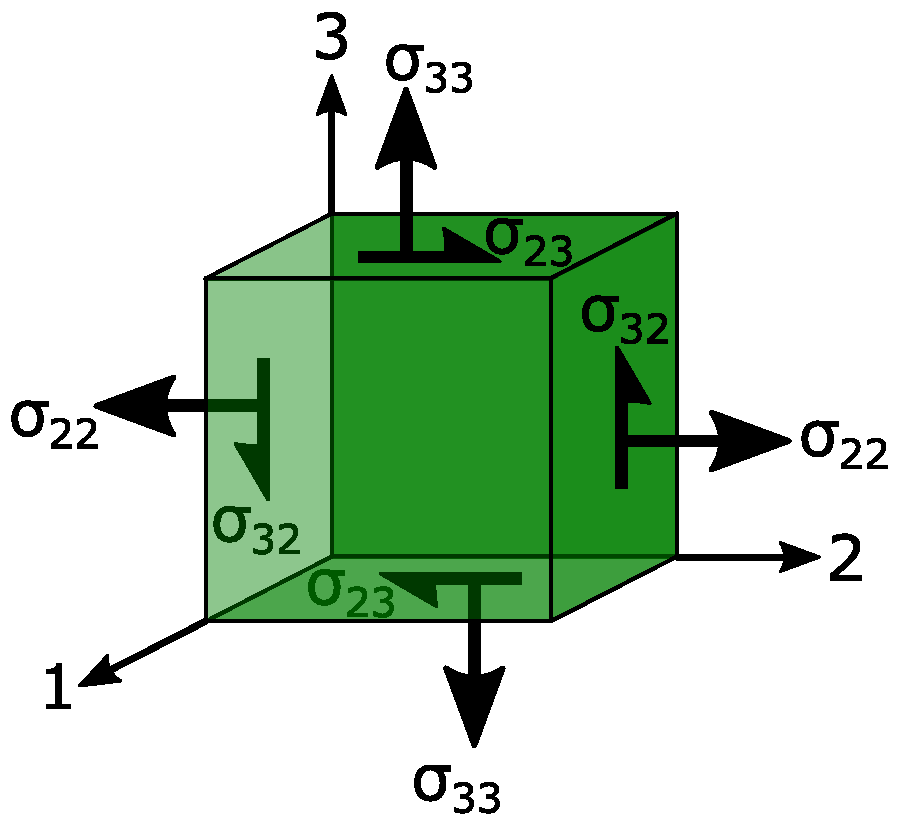
\includegraphics[width=0.66\textwidth]{Plane_Stress}
\caption{Illustration of the nomenclature of stresses acting on a body.\label{fig:plane_stress} }
\end{figure}

This nomenclature is shown for some of the possible stress components in \autoref{fig:plane_stress}. When thinking about stresses we assume that the body is in {\bf static equilibrium}, i.e. there are no net forces or moments acting on the body as a whole. 

This necessarily places constraints on the situation as depicted in \autoref{fig:plane_stress}. The simplest is that normal forces acting on opposite faces of the body must be equal, but for shear stresses there is a further constraint: not only must the forces on opposing faces be equal and opposite, e.g. the forces acting to give rise to $\sigma_{32}$, but also there must be a balance between the moments generated, such that $\sigma_{32} = \sigma_{23}$, preventing the rotation of the body under a net moment. This applies generally, so $\sigma_{ij} = \sigma_{ji}$, meaning that the stress tensor, \autoref{eqn:general_stress_tensor}, must be {\bf symmetrical}:
\\
\\

\begin{annotation}

\pgfdeclarelayer{background}
\pgfsetlayers{background,main}
{\centering
\begin{tikzpicture}
\centering
 \matrix[matrix of math nodes,left delimiter = (,right delimiter = ),row sep=10pt,column sep = 10pt] (m)
 {
\sigma_{11} & \sigma_{12} & \sigma_{13} \\
\sigma_{12} & \sigma_{22} & \sigma_{23} \\
\sigma_{13} & \sigma_{23} & \sigma_{33} \\
 };
\begin{pgfonlayer}{background}
 \draw[rounded corners,fill=green
,inner sep=3pt,fill opacity=0.3] (m-1-2.north west) -- (m-1-2.north east) -- (m-1-2.south east) -- (m-1-2.south west) -- (m-2-1.north east) -- (m-2-1.south east) -- (m-2-1.south west) -- (m-2-1.north west) -- (m-2-1.north east) -- (m-1-2.south west) -- cycle ;
 \draw[rounded corners,fill=green
,inner sep=3pt,fill opacity=0.3] (m-3-2.south east) -- (m-3-2.south west) -- (m-3-2.north west) -- (m-3-2.north east) -- (m-2-3.south west) -- (m-2-3.north west) -- (m-2-3.north east) -- (m-2-3.south east) -- (m-2-3.south west) -- (m-3-2.north east) -- cycle ;

 \draw[rounded corners,fill=green
,inner sep=3pt,fill opacity=0.3] (m-3-1.south east) -- (m-3-1.south west) -- (m-3-1.north west) -- (m-3-1.north east) -- (m-2-2.south west) -- (m-2-2.north west) -- (m-2-2.north east) -- (m-1-3.south west) -- (m-1-3.north west) -- (m-1-3.north east) -- (m-1-3.south east) -- (m-1-3.south west) -- (m-2-2.north east) -- (m-2-2.north west) -- (m-2-2.south west) -- (m-3-1.north east) -- cycle ;
\end{pgfonlayer}
\end{tikzpicture}
}

This means that only six components are required to fully define a stress state:

{\centering
\begin{tikzpicture}
\centering
 \matrix[matrix of math nodes,left delimiter = (,right delimiter = ),row sep=10pt,column sep = 10pt] (m)
 {
\sigma_{11} & \sigma_{12} & \sigma_{13} \\
\sigma_{12} & \sigma_{22} & \sigma_{23} \\
\sigma_{13} & \sigma_{23} & \sigma_{33} \\
 };
\begin{pgfonlayer}{background}
 \node[inner sep=3pt,fit=(m-1-1)]          (1)   {};
 \node[inner sep=3pt,fit=(m-1-2) (m-2-3)]  (2)   {};
 \node[inner sep=3pt,fit=(m-3-3)]          (3)   {};
 \draw[rounded corners,fill=green
,inner sep=3pt,fill opacity=0.3] (1.north west) -- (2.north east) |- (3.south west) |- (2.south west) |- (1.south west) -- cycle;
\end{pgfonlayer}
\end{tikzpicture}
}



BUT values depend on the reference axes.
\\
\\

\end{annotation}

\subsubsection{Axis Transformation}


There are six independent components of a general stress state, 3 normal stresses and 3 shear stresses. While the stress state itself must be unaffected by the choice of axes, the magnitude of these components will be affected, in much the same way as vectors. In fact, any tensor can be {\bf transformed} to refer to a new set of axes if the orientation relationship between the new set and old set of axes is known. 


The idea that the components of shear and normal stress vary with reference frame is not too difficult to understand. In \autoref{fig:shear_normal} it can be seen that two equal and perpendicular shear stresses in one frame of reference can be thought of as two equal and perpendicular normal stresses if the reference frame is rotated by \SI{45}{\degree}.


\begin{figure}[h!]
\centering
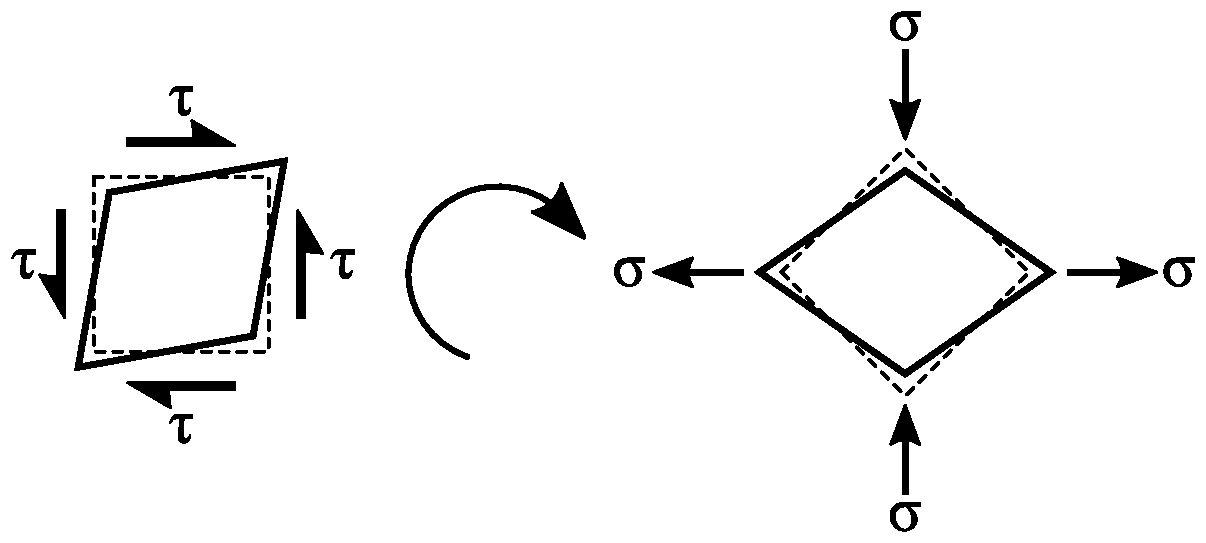
\includegraphics[width=0.6\textwidth]{shear_normal_equivalence}
\caption{Illustration that a pure shear stress state in one frame of reference can be represented by normal stresses in another.\label{fig:shear_normal}}
\end{figure}


This concept was partially discussed in IA course E when discussing slip systems and the resolved shear stresses.

\subsubsection*{Recap of Schmid Factor - See IA course E}


\begin{figure}[h!]
\centering
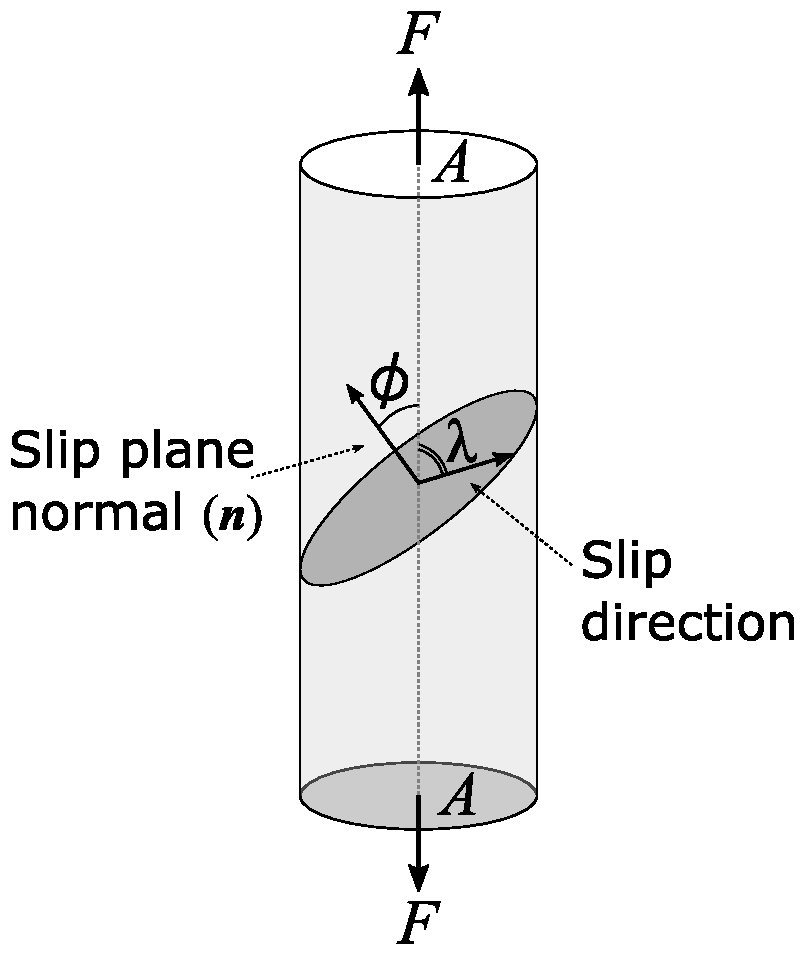
\includegraphics[width = 0.5\textwidth]{Schmid_Factor}
\caption{The geometry of the Schmid factor\label{fig:schmid_factor}}
\end{figure}

The Schmid factor is a method for calculating the shear component relevant to a particular slip system, i.e. the force acting along the slip direction and acting on the slip plane under the influence of a single applied tensile force.

By considering the slip system depicted in \autoref{fig:schmid_factor}, the component of the force parallel to the slip direction is $F\cos\lambda$, and the area of the plane is $A/\!\cos\phi$

This gives the resolved shear stress as:

\begin{equation}
\tau_\text{R} = \frac{F}{A} \cos \phi \cos \lambda \label{eqn:Schmid}
\end{equation}



The idea that the orientation being considered will affect the balance of normal can be intuitively understood

\FloatBarrier

Given a set of reference axes, \{1, 2, 3\}, a vector, $\mathbf{F}$, can be expressed as three components along each of these axes, $[F_1,\, F_2,\, F_3]$. If some other set of axes is defined, \{1', 2', 3'\}, then there will another representation of the vector  $\mathbf{F} = [F_{1'},\, F_{2'},\, F_{3'}]$. In \autoref{fig:axes_rotation} a vector is shown with respect to two axis sets that are related to each other by a rotation of $\phi$ about the 3 axis (which, therefore, coincides with the 3' axis).



\begin{figure}[h!]
\centering
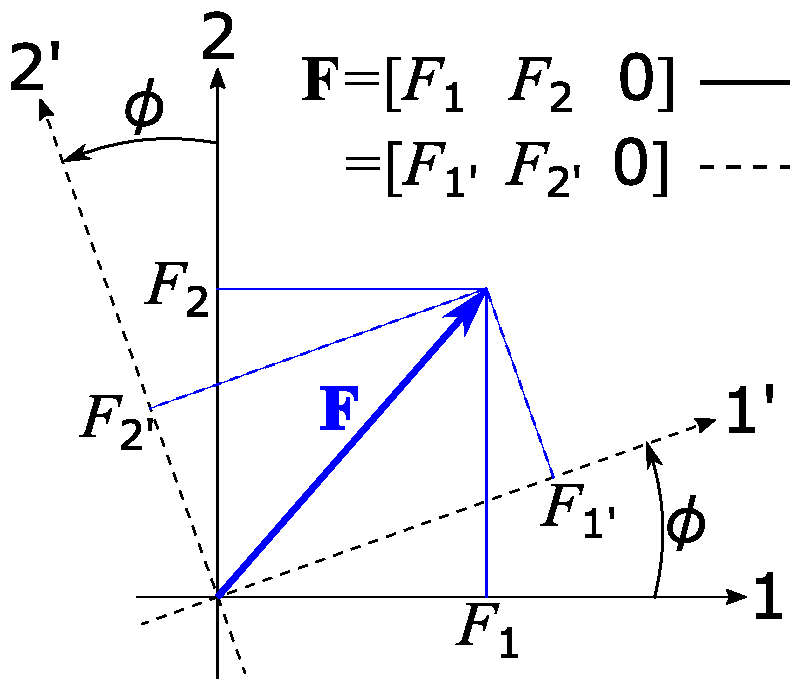
\includegraphics[width=0.6\textwidth]{rotate_axes}
\caption{Rotation, about the $3$ axis, of the axes defining the reference frame of a vector $\mathbf{F}$.\label{fig:axes_rotation}}
\end{figure}


The values of $F_{1'}$ and $F_{2'}$ can be found by resolving the components of $\mathbf{F}$, $F_2$ and $F_3$, along the 1' and 2' axes:

\begin{align}
F_{1'} &= F_1 \cos(1' \angle 1) + F_2 \cos(2' \angle 1) \nonumber\\
F_{2'} &= F_1  \cos(2' \angle 1) + F_2 \cos(2' \angle 2)
\end{align}

where the notation $(i' \angle j)$ indicates the angle between the $i'$ and $j$ axes.

In terms of $\phi$ this can be written:

\begin{align}
F_{1'} &= F_1 \cos(\phi) + F_2 \sin(\phi) \nonumber\\
F_{2'} &= - F_1  \sin(\phi) + F_2 \cos(\phi)
\end{align}

These trigonometric functions are key to transforming axes, and we can formulate a more general solution, known as direction cosines, the cosine of the angle from the new axis, $i'$, to the old axis, $j$:
\begin{annotation}
$$
a_{ij} = \cos(i' \angle j)
$$
\end{annotation}

This notation allows for rotation to be generalised to three dimensions:

\begin{align}
F_{1'}  &= a_{11}F_1 + a_{12} F_2 + a_{13} F_3 \nonumber\\
F_{2'}  &= a_{21}F_2 + a_{22} F_2 + a_{23} F_3 \\
F_{3'} &= a_{31}F_1 + a_{32} F_2 + a_{33} F_3 \nonumber
\end{align}

This can be written as a matrix operation:

\begin{equation}
\begin{bmatrix}
F_{1'} \\
F_{2'} \\
F_{3'}
\end{bmatrix} = 
\begin{bmatrix}
T
\end{bmatrix}
\begin{bmatrix}
F_1 \\ F_2 \\ F_3
\end{bmatrix}
\end{equation}
where the transformation matrix, $\begin{bmatrix}
T
\end{bmatrix}$, is given by:
\begin{equation}
\begin{bmatrix}
T
\end{bmatrix}
= \begin{bmatrix}
a_{11} & a_{12} & a_{13} \\
a_{21} & a_{22} & a_{23} \\
a_{31} & a_{32} & a_{33}
\end{bmatrix}
\end{equation}

For the transformation illustrated in \autoref{fig:axes_rotation} the transformation matrix would be:

\begin{equation}
\begin{bmatrix}
T
\end{bmatrix}
= \begin{bmatrix}
1 & 0 & 0 \\
0 & \cos\phi & \sin\phi \\
0 & -\sin\phi & \cos \phi
\end{bmatrix}
\end{equation}


This transformation matrix is similar to some you may have seen before when studying matrices in maths in previous years. You may notice that the sign of some of the terms is the opposite of what you expect, this is because we are rotating the reference frame, rather than the vector, effectively reversing the sign of the angle.

\subsubsection{Einstein summation convention}

These sorts of equations can be written more concisely, and more generally for higher order tensors, using the {\bf Einstein summation convention}. Whenever an index is repeated within a single term in an equation then a summation over all values of that index should be performed. Matrix multiplication provides a good example:

\begin{equation}
C_{ik} = A_{ij} B{jk} =  \sum_j A_{ij} B{jk} 
\end{equation}

where $j$ is a dummy suffix, i.e. it occurs twice in the term on the right hand side, and so we sum over all the possible values of $j=1,2,3$:

\begin{annotation}
\begin{equation}
C_{ik} = A_{i1}B_{1k} + A_{i2}B_{2k} + A_{i3}B_{3k}
\end{equation}
\end{annotation}


The example of a rotation above can be written:

\begin{equation}
F_{i'} = a_{ij}F_j
\end{equation}
\begin{annotation}
\centering
$j$ occurs twice
\end{annotation}

i.e. the first component of the force with respect to the new axes is:
\begin{equation}
F_{1'} = a_{11}F_1 + a_{12}F_2 + a_{13}F_3
\end{equation}
and so on for the other two components.
\\
\begin{annotation}
\begin{align*}
F_{2'} &= a_{21}F_1 + a_{22}F_2 + a_{23}F_3 \\
F_{3'} &= a_{31}F_1 + a_{32}F_2 + a_{33}F_3
\end{align*}
\end{annotation}
\\

To simplify the nomenclature this is often written with the prime on the symbol rather than the suffix to denote the transformed version:
\begin{equation}
F'_i = a_{ij}F_{j}
\end{equation}


This generalises to higher order tensors in a relatively straightforward manner:

\begin{equation}
\sigma'_{ij} = a_{ik} a_{jl} \sigma_{kl}
\end{equation}
\begin{annotation}
Apply the Einstein summation convention to $k$ and $l$
\end{annotation}
\\
\\

To illustrate this we can write the full equation for the $i=1$, $j=1$ component of $\sigma'_{ij}$:

\begin{align}
\sigma'_{11} =\,\,\, &a_{11}a_{11}\sigma_{11} + a_{11}a_{12}\sigma_{12} + a_{11}a_{13}\sigma_{13} \nonumber\\
 &a_{12}a_{11}\sigma_{21} + a_{12}a_{12}\sigma_{22} + a_{12}a_{13}\sigma_{23} \\
 &a_{13}a_{11}\sigma_{31} + a_{12}a_{13}\sigma_{23} + a_{13}a_{13}\sigma_{33} \nonumber
\end{align}



\begin{annotation}
Similarly for the 2-3 component:

\begin{align}
\sigma'_{23} =\,\,\, &a_{21}a_{31}\sigma_{11} + a_{21}a_{32}\sigma_{12} + a_{21}a_{33}\sigma_{13} \nonumber\\
                     &a_{22}a_{31}\sigma_{21} + a_{22}a_{32}\sigma_{22} + a_{22}a_{33}\sigma_{23} \nonumber \\
                     &a_{23}a_{31}\sigma_{31} + a_{22}a_{33}\sigma_{23} + a_{23}a_{33}\sigma_{33} \nonumber
\end{align}
And so on for the other components. c.f. Schmid law, \autoref{eqn:Schmid}, the shear is related to the normal stress by two direction cosines.

$$
\tau = \cos\phi \cos\lambda \sigma
$$
$$
\sigma_{23} = a_{21} a_{31} \sigma_{11}
$$

End of Lecture 1!
\end{annotation}
\\

\subsubsection{Principal stresses and strains, and the Secular Equation}

Using the transformations described above we can change a tensor to refer to new axes and change the values of the different components. Using this we can identify {\bf Principal Stresses }. These are normal stresses that act on {\bf Principal Planes}, which, by definition, have no shear stress acting upon them. A stress state expressed as principal stresses has the form:

\begin{equation}
\sigma_{ij} = \begin{annotation}
\begin{bmatrix}
\sigma_1 & 0 & 0 \\
0 & \sigma_2 & 0 \\
0 & 0 & \sigma_3
\end{bmatrix}\qquad
\text{where}\, \sigma_1,\,\, \sigma_2 \,\,\text{and}\,\, \sigma_3 \text{ are principal stresses}
\end{annotation}
\end{equation}

These are also the eigenvalues of the tensor. The single suffix is used to denote the fact that these are principal stresses. Obtaining the principal stresses is equivalent to diagonalising the tensor.

Second rank tensors are diagonalised in the same way as matrices, by solving the {\bf secular equation} (see a mathematics textbook for the derivation):

\begin{align}
\left|\sigma_{ij} - \lambda \mathbf{I} \right| = 0\qquad \begin{annotation}
\text{where {\bf I} is a unit matrix}
\end{annotation} \nonumber\\
\left| \begin{matrix}
\sigma_{11} - \lambda & \sigma_{12} & \sigma_{13} \\
\sigma_{21} & \sigma_{22} - \lambda & \sigma_{23} \\
\sigma_{31} & \sigma_{32} & \sigma_{33} - \lambda
\end{matrix}\right| = 0 \label{eqn:secular_equation}
\end{align}

To solve this equation we must use the determinant of a matrix:
\\

\begin{annotation}
$2 \times 2$
$$
A = \begin{bmatrix}
a & b \\
c & d
\end{bmatrix} \qquad \qquad \text{det} A = |A| = ad - bc
$$

$3\times3$

$$
|A| = \left| \begin{matrix}
a & b & c \\
d & e & f \\
g & h & i
\end{matrix} 
\right| = a \left| 
\begin{matrix} 
e & f \\ h & i\end{matrix} \right|
- b \left| 
\begin{matrix} 
d & f \\ g & i\end{matrix} \right|
+ c \left| 
\begin{matrix}
d & e \\
g & h
\end{matrix}
\right|
$$
\end{annotation}



For equation~\ref{eqn:secular_equation}, this gives a cubic equation for $\lambda$, each root of which is a principle stress. Using the determinant the secular equation becomes:

\begin{equation}
(\sigma_{11} - \lambda)[(\sigma_{22} - \lambda)(\sigma_{33}-\lambda) - \sigma_{23}^2] - \sigma_{12}[\sigma_{12}(\sigma_{33}-\lambda)-\sigma_{23}\sigma_{13}] + \sigma_{13}[\sigma_{12}\sigma_{13} - (\sigma_{22}-\lambda)\sigma_{13}] = 0
\end{equation}
This can be written:
\begin{equation}
\lambda^3 - I_1 \lambda^2 + I_2 \lambda - I_3 = 0 \label{eqn:cubic_roots}
\end{equation}
where
\begin{align}
I_1 &= \sigma_{11} + \sigma_{22} + \sigma_{33} \nonumber \\
I_2 &= \sigma_{11} \sigma_{22} + \sigma_{22} \sigma_{33} + \sigma_{33} \sigma_{11} - \sigma_{12}^2 - \sigma_{23}^2 - \sigma_{31}^2 \\
I_3 &= \sigma_{11}\sigma_{22}\sigma_{33} + 2\sigma_{12}\sigma_{23}\sigma_{31} - \sigma_{11} \sigma_{23}^2 - \sigma_{22}\sigma_{13}^2 - \sigma_{33}\sigma_{12}^2 \nonumber
\end{align}

These coefficients are called the invariants of the stress (or any other) tensor. They are not changed by a transformation of axes. A general stress state requires solving the cubic equation~\ref{eqn:cubic_roots}, though often things are simplified if one of the principle stress is already know, as this reduces the problem to a two-dimensional one.



\subsection{Mohr's Circle}

While finding the principal stresses by solving the secular equation is straightforward (if tedious), most problems involving stress states are not likely to be so generalised. It is quite common to know the magnitude and orientation of one principal stress and the corresponding plane, but to have more interest in principal directions within that plane, perhaps in how the normal and shear stresses vary with orientation within that plane.

If this is the case, and one root of the cubic secular equation is known then the problem reduces to a quadratic equation which can be solved via a geometrical construction, called Mohr's circle, which dates back to 1892 and was proposed by the German civil engineer Christian Otto Mohr.

If the 1-2 plane is a principal plane (i.e.\ $\sigma_{33}$ is a principal stress, and therefore $\sigma_{13} = \sigma_{23} = 0$) then the secular equation becomes:
\begin{equation}
\left| \begin{matrix}
\sigma_{11} - \lambda & \sigma_{12} & 0 \\
\sigma_{12} & \sigma_{22} - \lambda & 0 \\
0 & 0 & \sigma_{33}-\lambda
\end{matrix}\right| = 0
\end{equation}
remembering that $\sigma_{ij} = \sigma_{ji}$.

This becomes:
\begin{align}
(\sigma_{33}- \lambda)[(\sigma_{11} - \lambda)(\sigma_{22} - \lambda) - \sigma_{12}^2] = 0 \nonumber \\
\implies \lambda^2 - (\sigma_{11} + \sigma_{22})\lambda + (\sigma_{11}\sigma_{22} - \sigma_{12}^2) = 0
\end{align}

If we denote the two roots of this equation $\sigma_1$ and $\sigma_2$, we can write the solution as:

\begin{equation}
\sigma_1, \sigma_2 = \left( \frac{\sigma_{11} + \sigma_{22}}{2} \right) \pm \,\sqrt[]{\left( \frac{\sigma{11}-\sigma_{22}}{2}\right)^2 + \sigma_{12}^2} \label{eqn:Mohrs_circle_equation}
\end{equation}

The form of equation~\ref{eqn:Mohrs_circle_equation} can be interpreted graphically, where the first term defines the circles centre and the second term defines the radius. The circle would then be plotted with normal stresses along the horizontal axis and shear strains along the vertical axis.

\begin{figure}[hb!]
\centering
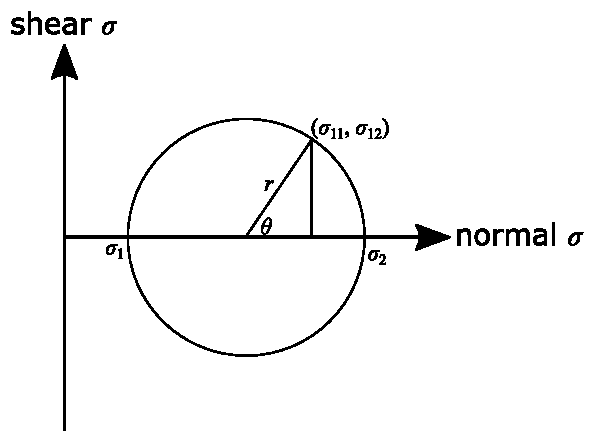
\includegraphics[width=0.5\textwidth]{Mohrs_Circle}
\caption{The graphical representation of the variation in normal and shear stresses as the frame of reference is rotated about a perpendicular principal axis.}
\end{figure}

\begin{annotation}
From this we can say:
\begin{equation}
r = \sqrt[]{\left( \frac{\sigma{11}-\sigma_{22}}{2}\right)^2 + \sigma_{12}^2} \qquad \qquad \tan \theta = \frac{2\sigma_{12}}{\sigma_{11} - \sigma_{22}}
\end{equation}
\end{annotation}

These results are derivable from the general transformation of tensors:
\begin{equation}
\sigma_{ij}' = a_{ik}a_{jl}\sigma_{kl}
\end{equation}
Since the 3 axis is a principal axis, we know $\sigma_{3}$ is a principal stress, and $\sigma_{13}=\sigma_{31}=0$ and $\sigma_{23}=\sigma_{32}=0$, this is simpler than the general case. If the transformation is:

\begin{equation}
a_{ij} = \left[ \begin{matrix}
\cos\phi & \sin\phi & 0 \\
-\sin\phi & \cos\phi & 0  \\
0 & 0 & 1
\end{matrix} \right]
\end{equation}
then the stresses are given by:
\begin{align}
\sigma_{11}' &= \cos^2\phi \sigma_1 + \sin^2\phi \sigma_2 \nonumber \\
\sigma_{22}' &= \sin^2\phi \sigma_1 + \cos^2\phi \sigma_2 \\
\sigma_{12}' &= - \sin\phi\cos\phi \sigma_1 + \sin \phi \cos \phi \sigma_2 \nonumber
\end{align}


These can be rearranged using trigonometric identities to be in terms of $2\phi$:

\begin{align}
\sigma_{11}' &= \left(\frac{\sigma_1 + \sigma_2}{2} \right) + \left( \frac{\sigma_1 - \sigma_2}{2} \right)\cos 2\phi \nonumber \\
\sigma_{22}' &= \left( \frac{\sigma_1 + \sigma_2}{2} \right) - \left( \frac{\sigma_1 - \sigma_2}{2} \right)\cos 2 \phi \\
\sigma_{12}' &= - \left( \frac{\sigma_1 - \sigma_2}{2}\right) \sin 2\phi
\end{align}

These equations can be solved with the circle construction above, where $2\phi = \theta$. The stress components (normal and shear) are given by the coordinates of a point on the circumference of the circle. As the frame of reference is rotated by an angle $\phi$, the point rotates around the circumference of the circle by an angle of $2\phi$. The circle is defined by the two principal stresses in question (here $\sigma_1$ and $\sigma_2$, the centre lies at the mean of the two principal stresses and the radius is half of the difference between the two principal stresses.

\begin{figure}[h!]
    \centering
    \begin{subfigure}{0.45\textwidth}
        \centering
        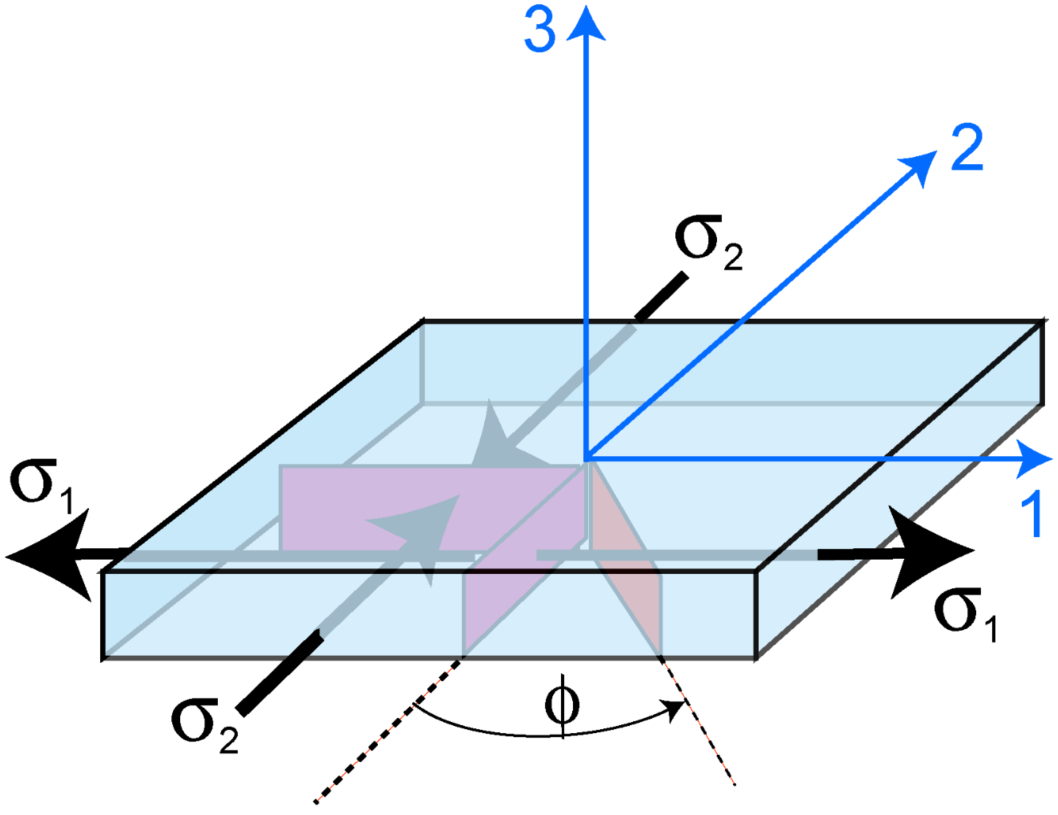
\includegraphics[width=\textwidth]{Real_space_rotate}
        \caption{}
    \end{subfigure}
~
    \begin{subfigure}{0.45\textwidth}
        \centering
        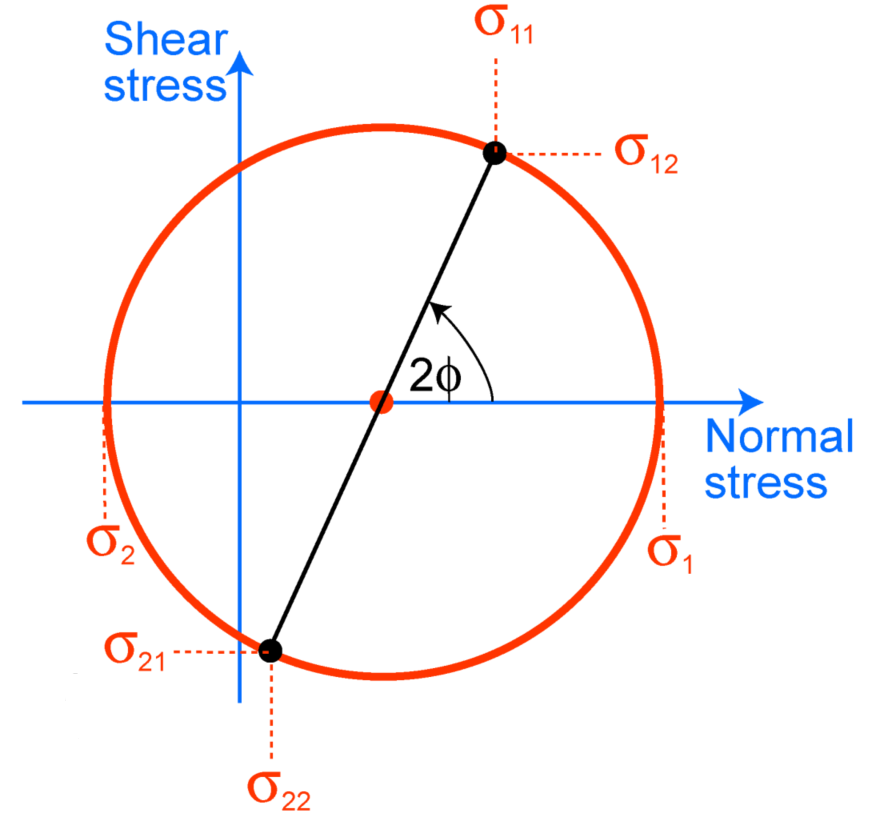
\includegraphics[width=\textwidth]{mohrs_circle_rotate}
        \caption{}
    \end{subfigure}
    \caption{Starting from a frame of reference where all the stresses are principal, i.e.\ a tension parallel to the 1-axis, a compression parallel to the 2-axis and no stress parallel to the 3-axis (a), the Mohr's circle construction allows us to calculate the stress components (both normal and shear) as the frame of reference is rotated. Note that this relies on the assumption that the 3 direction is a principal direction or equivalently that $\sigma_3$ is a principal stress.
    }
\end{figure}


\begin{annotation}
Conventions:
\begin{itemize}
\item Tensile stresses (normal by definition) are positive.
\item Compressive stresses (also normal) are negative.
\item There is no physical meaning to the sign of a shear stress, but clearly can \emph{change} sense if a force is reversed.
\end{itemize}
\end{annotation}



\subsubsection{Constructing Mohr's Circle}

Mohr's circle is a convenient graphical representation of the transformation of rotating the frame of reference about a principal axis. It allows the determination of various useful quantities including the principal stresses, the maximum shear stress, or the particular normal and shear components at arbitrary orientations. One common use is to find the principal stresses, $\sigma_1$ and $\sigma_2$, given the values of $\sigma_{11}$, $\sigma_{22}$ and $\sigma_{12}$ in some other frame of reference.

\begin{itemize}
\item First, construct a graph with normal stress along the horizontal axis and shear stress along the vertical axis using the same scale for both. The convention is that positive shear is downwards, and positive normal stress point to the right.

\item Plot the points ($\sigma_{11}$, $-\sigma_{12}$) and ($\sigma_{22}$, $\sigma_{12}$) and connect them with a straight line. Where this line corsses the horizontal axis is the centre of the circle. The angle between this line and the horizontal axis is $2\phi$.

\item Draw a circle centred on ($\frac{\sigma_{11} + \sigma_{22}}{2}$, $0$) passing through the two points.
\item The principal stresses are located at the intersection of the circle with the horizontal axis. 
\item The maximum shear is located at the top and the bottom of the circle, the magnitude is equal to the radius, i.e.\ $\frac{\sigma_{11} - \sigma_{22}}{2}$.
\item The angle of the diameter with the horizontal axis, $2\phi$, is twice the real space rotation, $\phi$.
\item This construction works for any second rank tensor, e.g.\ strain.
\end{itemize}

\begin{figure}
\centering
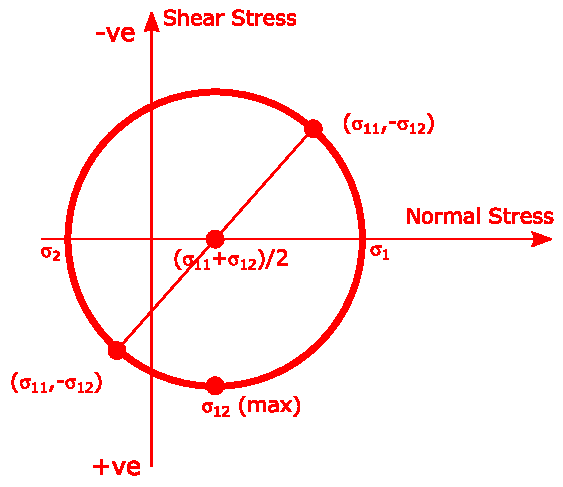
\includegraphics[height=7cm]{mohrs_circle_construction}
\end{figure}

\subsubsection{Examples of Mohr's circle}

(a) Uniaxial Tension, $\sigma_{11} = \sigma_{1}$

\begin{annotation}
$\sigma_{ij} = \begin{bmatrix}
\sigma_1 & 0 & 0 \\
0 & 0 & 0 \\
0 & 0 & 0
\end{bmatrix}$  \qquad 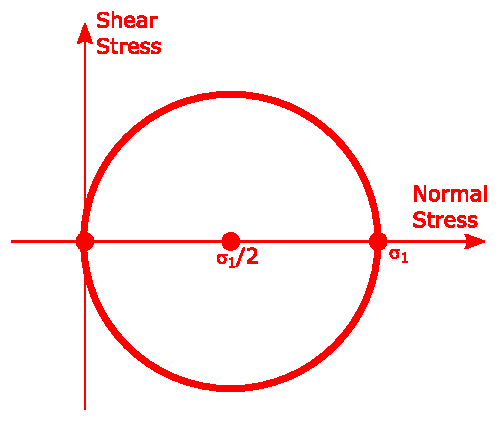
\includegraphics[width=6cm]{mohrs_uniaxial_tension}
\end{annotation}
\\

(b) Biaxial stress with equal compression and tension, $\sigma_{11} = \sigma_1, \sigma_{22}=-\sigma_1$

\begin{annotation}
$\sigma_{ij} = \begin{bmatrix}
\sigma_1 & 0 & 0 \\
0 & -\sigma_1 & 0 \\
0 & 0 & 0
\end{bmatrix}$  \qquad 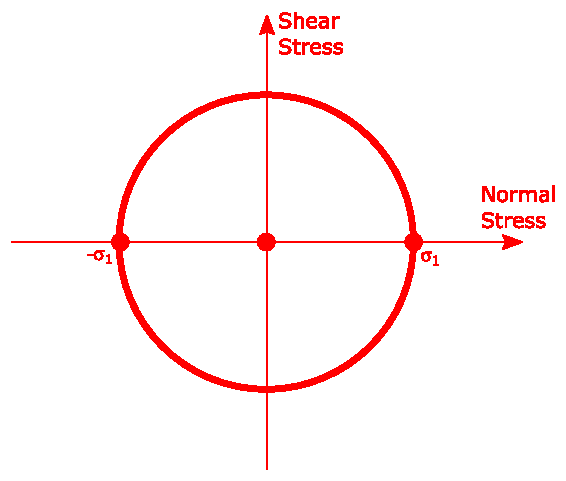
\includegraphics[width=6cm]{mohrs_biaxial_tension_compression}
\end{annotation}
\\
\begin{annotation}


We can represent the rotation of the frame of reference about each of the three principal axes:\\
{\hspace{4cm}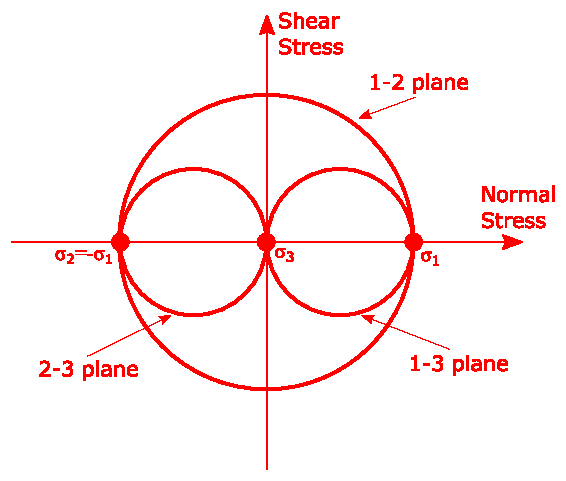
\includegraphics[width=6cm]{mohrs_biaxial_tension_compression_complete}}
\end{annotation}

(c) Triaxial Tension, $\sigma_{11}=\sigma_1, \sigma_{22}=\sigma_2, \sigma_{33}=\sigma_3$ (convention is that $\sigma_1>\sigma_2>\sigma_3$


\begin{annotation}
$\sigma_{ij} = \begin{bmatrix}
\sigma_1 & 0 & 0 \\
0 & \sigma_2 & 0 \\
0 & 0 & \sigma_3
\end{bmatrix}$  \qquad 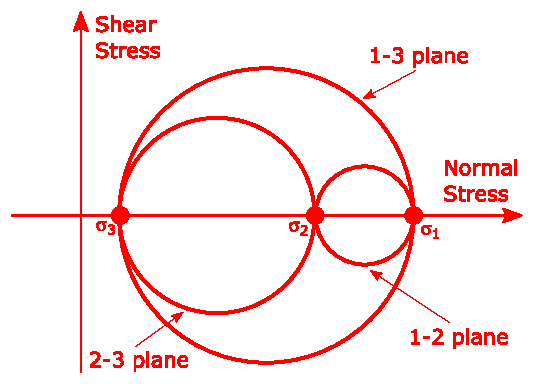
\includegraphics[width=6cm]{mohrs_triaxial_tension}
\end{annotation}
\\


% Example use of Mohr's circle here?

\subsection{Strain - a full treatment}

We have thus far dealt with stresses that arise due to applied forces on a material. These stresses cause deformations in a material, either reversible (elastic) or irreversible (plastic). We will first address the reversible strains, which tend to be limited to somewhat less than \SI{1}{\percent} (except in extreme cases like rubbery polymers).

Much like the stress tensor, the strain tensor must also be symmetrical. For stresses this removed the effect of net moments on a body, in the case of strains this is removing any rigid body rotation that is not associated with any deformation in the material itself. This is relevant to the simple deformation of shear strain given at the beginning of the course, which we will see includes a component of rotation.

\subsubsection{Relative displacement tensor}

Considering before and after a stress state is induced by  appling forces to a material, there will be resultant set of displacements of all points away from their initial positions. Assuming that the material is homogeneous, the displacements will be related to the stress state by the elastic properties of the material.

The \emph{relative displacement tensor} or \emph{deformation tensor} is a second rank tensor that defines how any point is displaced from it's initial position including normal and shear components in all three real space dimensions.

The components of the relative displacement tensor are defined by:
\begin{equation}
e_{ij} = \frac{\partial u_i}{\partial x_j}
\end{equation}
where $u_i$ is the displacement in the $i$th axis and $x_j$ is the position along the reference $j$th axis. These are dimensionless ratios of two distances. This is shown for the 2-3 plane in \autoref{fig:displacement_tensor}.
\FloatBarrier

\begin{figure}[h!]
\centering
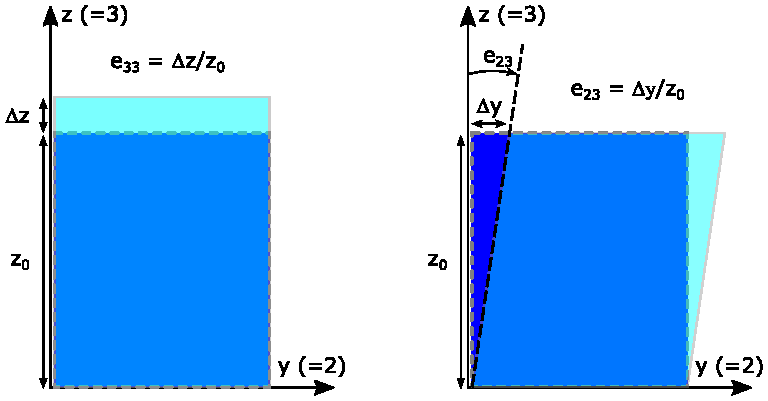
\includegraphics[width=0.8\textwidth]{displacement_tensor}
\caption{Illustration in the y-z (2-3) plane of how the relative displacement terms are defined. Note that $e_{23}$ (and other shear terms) can be considered angles when displacements are small. Conventionally the shear components are taken to be positive when the effect is to rotate the ositive reference axis towards the positive displacement axis, i.e. here rotating the positive 3-axis (reference) towards the positive 2-axis (displacement).\label{fig:displacement_tensor}}
\end{figure}

The definition of the shear term in \autoref{fig:displacement_tensor} is the same as the definition of simple shear given at the beginning of the course. However, this definition does not necessarily result in a symmetric tensor, in the situation shown in \autoref{fig:displacement_tensor} it is clear that $e_{23}\neq e_{32}$, since $e_{23}= \Delta y / z_0$ but $e_{32}=0$. Indeed, in general the displacement tensor is not constrained, and so is made up of two components, one symmetric component, strain, and one anti-symmetric component, rigid rotation, as shown in \autoref{fig:disp_strain_rotate}.


\FloatBarrier

\begin{figure}[h!]
\centering
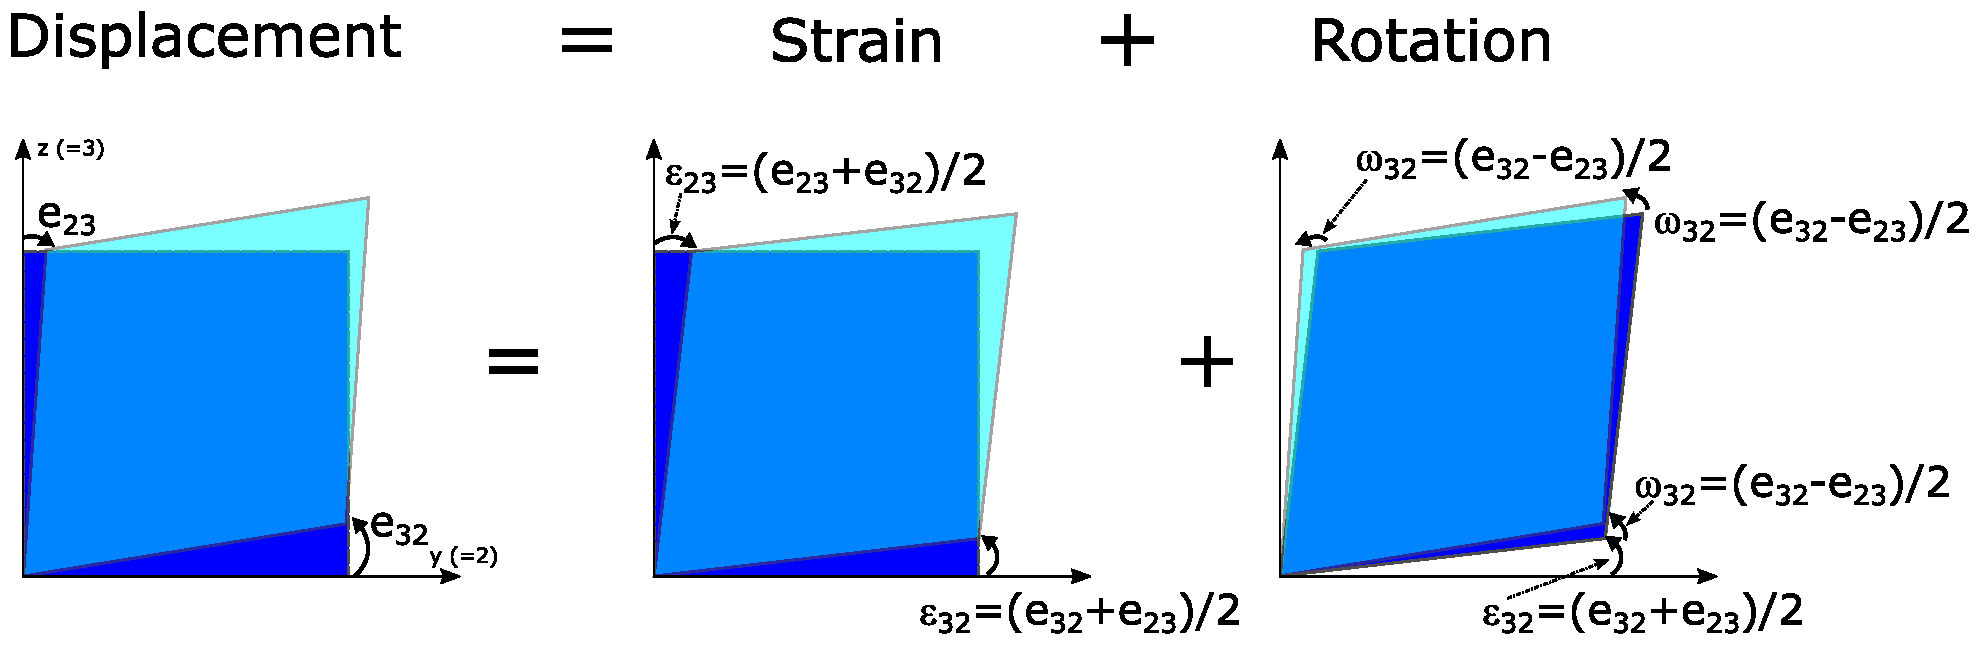
\includegraphics[width=\textwidth]{displacement_strain_rotation}
\caption{Schematic showing that a general displacements ($e_{23},e_{32}$) can be represented by  strains ($\varepsilon_{23} = \varepsilon_{32}$) and a rotation ($\omega_{23}=-\omega_{32}$).\label{fig:disp_strain_rotate}}
\end{figure}

\FloatBarrier

In general a second rank tensor can be expressed as a symmetric component and an antisymmetric component:\\
\begin{annotation}
\begin{equation}
e_{ij} = \dfrac{1}{2}(e_{ij} + e_{ji}) + \dfrac{1}{2}(e_{ij} - e_{ji}) \\
\end{equation}
\\
or for the specific case illustrated above:
\begin{equation}
e_{23} = \dfrac{1}{2}(e_{23} + e_{32}) + \dfrac{1}{2}(e_{23} - e_{32})
\end{equation}


Strain is the symmetric component: $\varepsilon_{ij}=\varepsilon_{ji}$\\
Rotation is the antisymmetric component: $\omega_{ij} = - \omega_{ji}$
\end{annotation}



 So the two components of a general displacement are:
\begin{align}
\text{Strain} \qquad \qquad & \qquad \qquad \text{Rotation} \nonumber \\
\varepsilon_{ij} = \dfrac{1}{2}(e_{ij} + e_{ji}) \qquad & \qquad \omega_{ij} = \dfrac{1}{2}(e_{ij} - e_{ji})
\end{align}

The definition of $\omega_{ij}$ means that itis antisymmetric and the leading diagonal is zero, and it easy to see that it represents a rigid body rotation, for example in 2D:
\begin{equation}
\omega_{ij} = \begin{bmatrix}
0 & \omega \\
-\omega & 0 
\end{bmatrix}
\end{equation}
results in a rotation:
\FloatBarrier
\begin{figure}[h!]
\centering
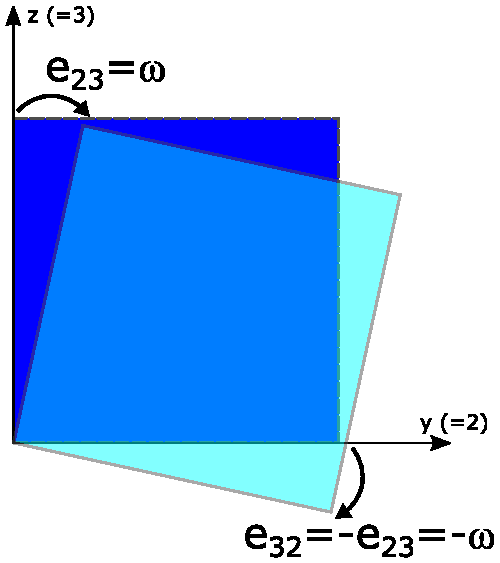
\includegraphics[width=0.5\textwidth]{rotation}
\caption{Schematic showing the rigid body rotation that arises from the anti-symmetric component of a general displacement tensor.}
\end{figure}
\FloatBarrier


Normally we do not consider the rigid body rotation further, it may be important from a structures point of view, but for the material itself it is not relevant.

Since strain is a second rank tensor, like the stress tensor it can be diagonalised to give the principal strains and like principal stresses, these are normal stresses that act in principal directions which experience no shear strain. The same matrix transformations apply and constructions like Mohr's circle can be used.

For completeness the full strain tensor is given by:
\begin{equation}
\begin{bmatrix}
\varepsilon_{11} & \varepsilon_{12} & \varepsilon_{13} \\
\varepsilon_{12} & \varepsilon_{22} & \varepsilon_{23} \\
\varepsilon_{13} & \varepsilon_{23} & \varepsilon_{33}
\end{bmatrix}
=
\begin{bmatrix}
e_{11} & ^1\!/_2 (e_{12} + e_{21}) & ^1\!/_2 (e_{13} + e_{31}) \\
^1\!/_2 (e_{21} + e_{12}) & e_{22} & ^1\!/_2 (e_{23} + e_{32}) \\
^1\!/_2 (e_{31} + e_{13}) & ^1\!/_2 (e_{32} + e_{23}) & e_{33}
\end{bmatrix}
\end{equation}
and when referred to principal axes this becomes:
\begin{equation}
\varepsilon_{ij} = \begin{bmatrix}
\varepsilon_1 & 0 & 0 \\
0 & \varepsilon_2 & 0 \\
0 & 0 & \varepsilon_3
\end{bmatrix}
\end{equation}


\subsubsection{Hydrostatic and deviatoric strains}

The strain tensor can be described as the sum of two components, a hydrostatic and deviatoric components. In broad terms the hydrostatic component is the strain associated with a change in volume and the deviatoric component is the strain associated with shape changes without any volume strain.

Considering an element of material subjected to principal strains $\varepsilon_1, \varepsilon_2$ and $\varepsilon_3$. The volumetric strain (see IA course E) can be written as:
\begin{equation}
\Delta = (1+\varepsilon_1)(1+\varepsilon_2)(1+\varepsilon_3) -1 = \varepsilon_1 + \varepsilon_2 + \varepsilon_3 + O(\varepsilon^2)
\end{equation}
The higher order terms can be ignored for small strains. This is equivalent to the trace of the tensor, and this is invariant under any transformation of reference axes, so this can be written succinctly in suffix notation:
\begin{equation}
\Delta = \varepsilon_{ii}
\end{equation}

The hydrostatic component of a general strain will therefore have the form:
\begin{equation}
\varepsilon_{ij} = \begin{bmatrix}
^{\Delta}\!/_3 & 0 & 0 \\
0 & ^{\Delta}\!/_3 & 0 \\
0 & 0 & ^{\Delta}\!/_3
\end{bmatrix}
\end{equation}
and the other component follows:
\begin{equation}
\begin{bmatrix}
\varepsilon_{11} & \varepsilon_{12} & \varepsilon_{13} \\
\varepsilon_{12} & \varepsilon_{22} & \varepsilon_{23} \\
\varepsilon_{13} & \varepsilon_{23} & \varepsilon_{33}
\end{bmatrix}
= \begin{bmatrix}
\Delta/3 & 0 & 0 \\
0 & \Delta3 & 0 \\
0 & 0 & \Delta/3
\end{bmatrix}
+ \begin{bmatrix}
\varepsilon_{11} - ^{\Delta}\!/_3 & \varepsilon_{12} & \varepsilon_{13} \\
\varepsilon_{12} & \varepsilon_{22} - ^{\Delta}\!/_3 & \varepsilon_{23} \\
\varepsilon_{13} & \varepsilon_{23} & \varepsilon_{33} - ^{\Delta}\!/_3
\end{bmatrix}
\end{equation}

\begin{annotation}
\qquad\qquad General strain \qquad\quad hydrostatic \qquad\qquad\qquad\qquad deviatoric
\end{annotation}

The effects of these individual components are shown schematically in \autoref{fig:strain_components}.
\begin{figure}
\centering
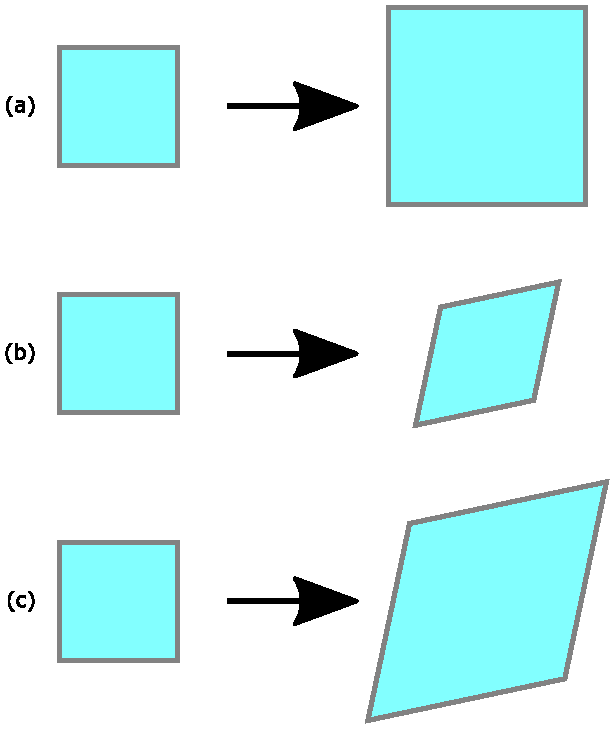
\includegraphics[width=0.5\textwidth]{strain_components}
\caption{Schematic showing the effects of (a) a hydrostatic strain, (b) a deviatoric strain and (c) a general strain made up of both components.\label{fig:strain_components}}
\end{figure}


\subsubsection{Shear strain - engineering vs tensor definitions}

There is a minor complication in our descriptions of shear strains. Our tensor definition includes shear terms, for example $\varepsilon_{12}$, so it might be expected that the shear modulus would be defined by the ratio of $\varepsilon_{12}/\sigma_{12}$. Unfortunately $G\neq \varepsilon_{12}/\sigma_{12}$. The problem is to do with our original definition of the shear modulus, see \autoref{eqn:def_moduli}. We might write this with suffices as:
\begin{equation}
G=\frac{\sigma_{12}}{\gamma_{12}} \qquad \qquad \qquad \begin{annotation}
G = \frac{\tau}{\gamma}
\end{annotation}
\end{equation}
where $\gamma_{12}$ is the simple strain, with  no account made for the fact that this should be represented as two shear strains ($\varepsilon_{12}=\varepsilon_{21}$) and a rigid body rotation ($\omega_{12}=-\omega_{21}$). This is shown in \autoref{fig:tensor_vs_engineer_shear}.
\FloatBarrier
\begin{figure}
\centering
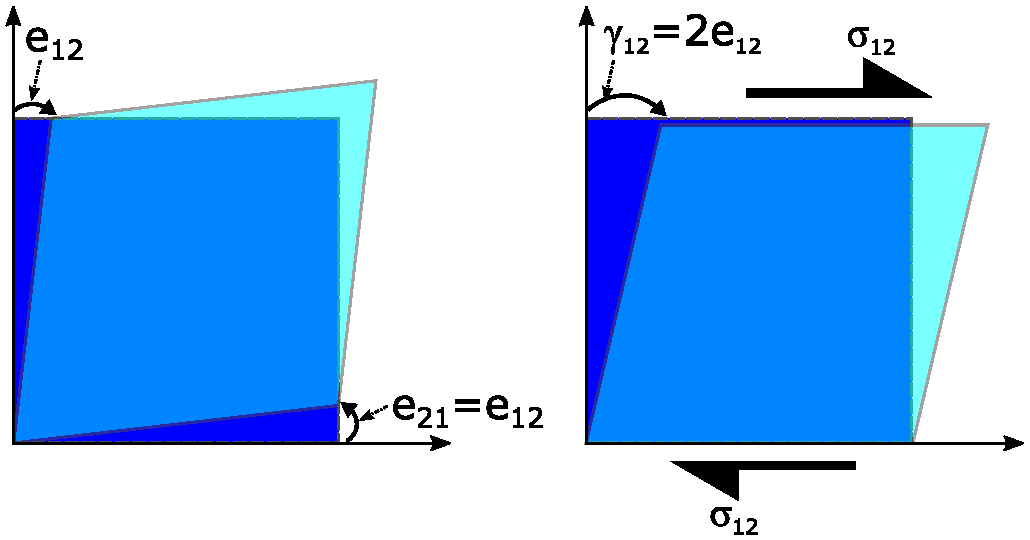
\includegraphics[width=0.6\textwidth]{tensor_vs_engineering_shear}
\caption{Schematic showing the difference between tensor shear (left) where two components describe the shape change, and there is no rotation, and engineering shear, right, where a single component describes the shear and includes an implicit rotation.\label{fig:tensor_vs_engineer_shear}}
\end{figure}
\FloatBarrier
This means that the shear modulus is instead defined by the equation:
\begin{equation}
G=\frac{\sigma_{12}}{\gamma_{12}}
\end{equation}
and that the engineering strains, $\varepsilon_{ii}$ and $\gamma_{ij}$, do not form a tensor and therefore can't be manipulated using tensor methods discussed here, such as axis transformation or relation to stress via the stiffness or compliance tensor. That said, the simple shear modulus can be related to the tensor formulation:

\begin{align}
\varepsilon_{12} = S_{1212}\sigma_{12} + S_{1221}\sigma_{21} = 2 S_{1212}\sigma_{12}\nonumber \\
 G = \frac{\sigma_{12}}{\gamma_{12}} = \frac{\sigma_{12}}{2\varepsilon_{12}} = \frac{1}{4S_{1212}}
\end{align}

For isotropic materials this sort of analysis can be done to link simple elastic engineering constants (Young's modulus, bulk modulus, shear modulus, Poisson ratio etc.) with the components of the compliance and stiffness tensors. In fact there are only two independent constants so $E$ and $\nu$ are sufficient. Where materials are anisotropic there are more independent components and the analysis becomes more difficult.



\subsection{Stiffness and Compliance}

We are used to the idea that in a simple uniaxial stress state the strain is linked to stress by the equation:
\begin{equation}
\sigma = E \varepsilon
\end{equation}
when using stress and strain tensors for general cases this relationship becomes:
\begin{equation}
\sigma_{ij} = C_{ijkl}\varepsilon_{kl} \label{eqn:hookes_law}
\end{equation}
where $C_{ijkl}$ is called the stiffness tensor. Since both stress and strain are second rank tensors, and all the components of strain could have a dependence on all the components of stress the stiffness is a fourth rank tensor (in general a tensor that relates an $n$th rank and an $m$th rank tensor will have a rank of $n+m$). The stiffness will therefore have $3\times3\times3\times3$ components (81!).  

\autoref{eqn:hookes_law} is the generalised form of Hooke's law, and materials that obey this are said to be \emph{linearly elastic}. The inverse relationship can be written:
\begin{equation}
\varepsilon_{ij} = S_{ijkl} \sigma_{kl}
\end{equation}
where $S_{ijkl}$ is the compliance tensor. (Note the annoying convention that the letters representing stiffness and compliance are the reverse of the initial letter of each word.)

\subsubsection{Constraints on the stiffness tensor}

In principal there are a large number of terms to deal with for a general stress state and this is tedious if not daunting, however there are various constraints that limit the number of terms that need to be considered in most cases.

One constraint that always applies is that the body is in static equilibrium, and as a result the stress and strain tensors are symmetrical, such that $\sigma_{ij}=\sigma_{ji}$ and $\varepsilon_{kl}=\varepsilon_{lk}$. Thus the $i$ and $j$ indices can be swapped without effect, and similarly $k$ and $l$. This means that:
\begin{equation}
C_{ijkl}=C_{jikl}=C_{ijlk}=C_{jilk}
\end{equation}
This reduces the components from 81 to 36. Furthermore there is usually some symmetry inherent to the material that reduces this number further, for example the response of a cubic material to an applied stress will not vary under a transformation that maps [1\,0\,0] to the [0\,1\,0]. For a cubic material there are only three independent elastic constants. For a completely isotropic material, like glass or a randomly oriented polycrystal there re only 2 independent elastic constants.

\subsubsection{Relationship to Young's modulus}

It is tempting to relate the tensor stiffness to elastic constants by considering  the application of one normal stress and a single normal strain arising as a result:
\begin{equation}
\sigma_{11} = E \varepsilon_{11}
\end{equation}
where $E$ is the Young's modulus which we are familiar with. From this one might conclude that $C_{1111}=E$. This is not correct though, because the application of a single stress does not give rise to a single strain due to Poisson strains:
\FloatBarrier
\begin{figure}[h!]
\centering
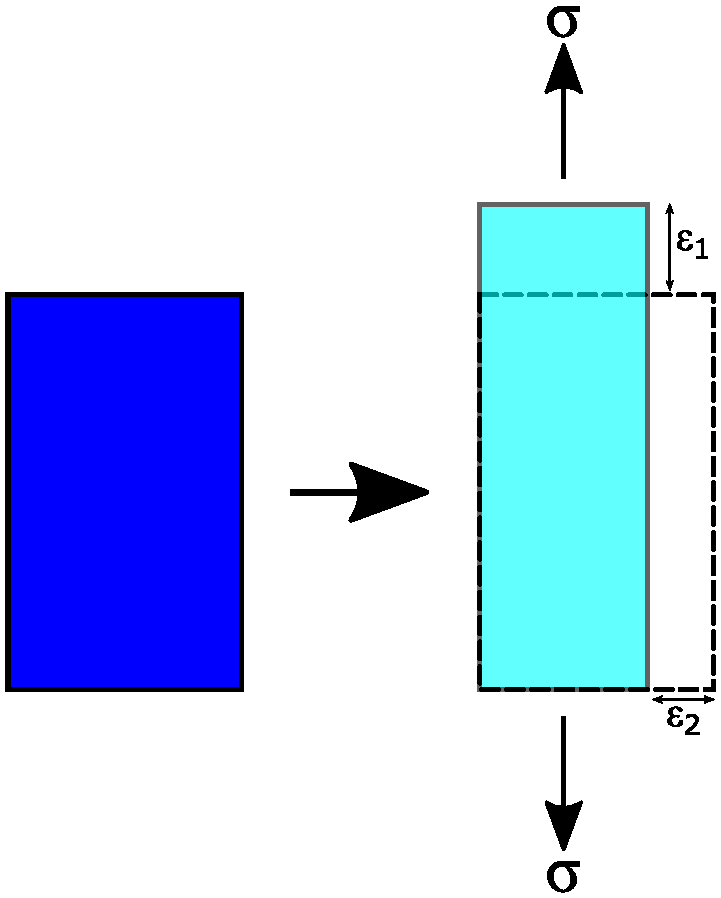
\includegraphics[width=4cm]{poisson_strains}
\end{figure}
\FloatBarrier

This means that there are in fact three strain terms that depend on the single stress in the full tensor description of the situation. However, if we instead consider this in terms of compliance then Young's modulus can be related to the tensor elastic constants:
\begin{equation}
\varepsilon_{11} = S_{1111}\sigma_{11}
\end{equation}
Now there is only one stress term and ne strain term relevant to the equation and therefore Young's modulus is:
\begin{equation}
E = \frac{1}{S_{1111}}
\end{equation}

\subsubsection{Relationship to the Poisson ration}

The Poisson ratio, represented by the symbol $\nu$, gives the transverse contraction that arises as a result of a axial tensile strain. Considering the application of a single normal stress, $\sigma_{1}$ generating principal strains $\varepsilon_1, \varepsilon_2$ and $\varepsilon_3$, the Poisson ratio is defined to be:
\begin{equation}
\varepsilon_2 = -\nu \varepsilon_1 \label{eqn:poisson_definition}
\end{equation}
and in tensor notation we can write:
\begin{equation}
\epsilon_2 = S_{2211}\sigma_1 \begin{annotation}
= S_{1122}\sigma_1
\end{annotation}
\end{equation}

Using the definition of Young's modulus we can substitute for $\varepsilon_1$ in \autoref{eqn:poisson_definition}:
\begin{equation}
\varepsilon_2 = -\nu \frac{\sigma_1}{E}
\end{equation}
and substituting for $\varepsilon_2$:
\begin{equation}
S_{1122} \sigma_1 = -\frac{\nu}{E} \sigma_1
\end{equation}
so
\begin{equation}
S_{1122} = -\frac{\nu}{E}
\end{equation}

During multiaxial loading (i.e.\ with more than one non-zero principal stress) the Poisson strains superimpose this leads to a set of equations for the principal strains that arise from an applied set of principal stresses (for an isotropic material):
\begin{align}
\varepsilon_1 = \frac{\sigma_1}{E} - \nu \frac{(\sigma_2 + \sigma_3)}{E} \nonumber\\
\varepsilon_2 = \frac{\sigma_2}{E} - \nu \frac{(\sigma_1 + \sigma_3)}{E}  \label{eqn:constitutive_laws}\\
\varepsilon_3 = \frac{\sigma_3}{E} - \nu \frac{(\sigma_1 + \sigma_2)}{E} \nonumber 
\end{align}
































































